\section{Рабочий проект}
\subsection{Классы, используемые при разработке серверной части программной системы}

В данном разделе описывается список классов и их методов, использованных при разработке серверной части программной системы. 

\subsubsection{Спецификация классов SQL запросов}

Основные SQL-классы для подключения к базе данных включают SQLConnectionDb и DatabaseManager. 

SQLConnectionDb предоставляет методы для управления соединением с базой данных, включая открытие, закрытие и проверку состояния соединения. Этот класс используется для синхронного взаимодействия с базой данных.

DatabaseManager - это асинхронная версия класса подключения к базе данных, которая обеспечивает возможность выполнения асинхронных запросов к базе данных для улучшения производительности и масштабируемости. Он предоставляет асинхронные версии методов для работы с соединением, что позволяет выполнять асинхронные операции базы данных без блокировки потока.

В таблицах 4.1 -- 4.19 приведено описание полей и методов классов для работы с базой данных.

\renewcommand{\arraystretch}{0.8} % уменьшение расстояний до сетки таблицы
\begin{xltabular}{\textwidth}{|X|p{3cm}|p{3cm}|>{\setlength{\baselineskip}{0.7\baselineskip}}p{4.85cm}|}
	\caption{Спецификация полей класса «SQLConnectionDb» \label{class1:table}}\\
	\hline \centrow \setlength{\baselineskip}{0.7\baselineskip} Наименование & \centrow \setlength{\baselineskip}{0.7\baselineskip} Метод доступа & \centrow Тип данных & \centrow Описание \\
	\hline \centrow 1 & \centrow 2 & \centrow 3 & \centrow 4\\ \hline
	\endfirsthead
	\continuecaption{Продолжение таблицы \ref{class1:table}}
	\centrow 1 & \centrow 2 & \centrow 3 & \centrow 4\\ \hline
	\finishhead
	connectionString & private & string? & Строка подключения к БД \\ \hline 
	connection & protected & SqlConnection & Состояние подключения к БД \\ \hline 
\end{xltabular}
\renewcommand{\arraystretch}{1.0} % восстановление сетки

\renewcommand{\arraystretch}{0.8} % уменьшение расстояний до сетки таблицы
\begin{xltabular}{\textwidth}{|p{4cm}|p{3cm}|>{\setlength{\baselineskip}{0.7\baselineskip}}X|}
	\caption{Спецификация методов класса «SQLConnectionDb» \label{class2:table}}\\
	\hline \centrow \setlength{\baselineskip}{0.7\baselineskip} Наименование & \centrow \setlength{\baselineskip}{0.7\baselineskip} Метод доступа & \centrow Описание \\
	\hline \centrow 1 & \centrow 2 & \centrow 3\\ \hline
	\endfirsthead
	\continuecaption{Продолжение таблицы \ref{class2:table}}
	\centrow 1 & \centrow 2 & \centrow 3\\ \hline
	\finishhead
	ConnectionDB & public & Устанавливает соединение с базой данных, используя заданную строку подключения. В случае успеха возвращает объект типа SqlConnection, представляющий активное соединение. В случае ошибки выводит сообщение об ошибке и возвращает null.\\ \hline 
	CloseDB & public & Закрывает текущее соединение с базой данных. Не принимает аргументов. Возвращает объект типа SqlConnection, представляющий закрытое соединение.\\ \hline 
\end{xltabular}
\renewcommand{\arraystretch}{1.0} % восстановление сетки

\renewcommand{\arraystretch}{0.8} % уменьшение расстояний до сетки таблицы
\begin{xltabular}{\textwidth}{|X|p{3cm}|p{3cm}|>{\setlength{\baselineskip}{0.7\baselineskip}}p{4.85cm}|}
	\caption{Спецификация полей класса «DatabaseManager» \label{class3:table}}\\
	\hline \centrow \setlength{\baselineskip}{0.7\baselineskip} Наименование & \centrow \setlength{\baselineskip}{0.7\baselineskip} Метод доступа & \centrow Тип данных & \centrow Описание \\
	\hline \centrow 1 & \centrow 2 & \centrow 3 & \centrow 4\\ \hline
	\endfirsthead
	\continuecaption{Продолжение таблицы \ref{class3:table}}
	\centrow 1 & \centrow 2 & \centrow 3 & \centrow 4\\ \hline
	\finishhead
	connectionString & private static & string & Строка подключения к БД \\ \hline 
\end{xltabular}
\renewcommand{\arraystretch}{1.0} % восстановление сетки

\renewcommand{\arraystretch}{0.8} % уменьшение расстояний до сетки таблицы
\begin{xltabular}{\textwidth}{|p{4cm}|p{3cm}|>{\setlength{\baselineskip}{0.7\baselineskip}}X|}
	\caption{Спецификация методов класса «DatabaseManager» \label{class4:table}}\\
	\hline \centrow \setlength{\baselineskip}{0.7\baselineskip} Наименование & \centrow \setlength{\baselineskip}{0.7\baselineskip} Метод доступа & \centrow Описание \\
	\hline \centrow 1 & \centrow 2 & \centrow 3\\ \hline
	\endfirsthead
	\continuecaption{Продолжение таблицы \ref{class4:table}}
	\centrow 1 & \centrow 2 & \centrow 3\\ \hline
	\finishhead
	OpenConnection Async & public async & Асинхронно открывает соединение с базой данных, используя строку подключения. Возвращает объект типа SqlConnection, представляющий активное соединение.\\ \hline 
	CloseConnection Async & public async & Асинхронно закрывает указанное соединение с базой данных, если оно открыто. Не принимает аргументов.\\ \hline 
\end{xltabular}
\renewcommand{\arraystretch}{1.0} % восстановление сетки

\renewcommand{\arraystretch}{0.8} % уменьшение расстояний до сетки таблицы
\begin{xltabular}{\textwidth}{|p{4cm}|p{3cm}|>{\setlength{\baselineskip}{0.7\baselineskip}}X|}
	\caption{Спецификация методов класса «SQLCar» \label{class6:table}}\\
	\hline \centrow \setlength{\baselineskip}{0.7\baselineskip} Наименование & \centrow \setlength{\baselineskip}{0.7\baselineskip} Метод доступа & \centrow Описание \\
	\hline \centrow 1 & \centrow 2 & \centrow 3\\ \hline
	\endfirsthead
	\continuecaption{Продолжение таблицы \ref{class6:table}}
	\centrow 1 & \centrow 2 & \centrow 3\\ \hline
	\finishhead
	AddCar & public & Добавляет новую запись о машине в базу данных. Принимает объект типа Car в качестве аргумента. Возвращает логическое значение, указывающее на успешность операции добавления.\\ \hline 
	GetCarsByUser & public & Возвращает список машин, принадлежащих определенному пользователю. Принимает номер телефона пользователя в качестве аргумента. Возвращает список объектов типа Car.\\ \hline 
	DeleteCar & public & Удаляет запись о машине из базы данных. Принимает номер телефона пользователя и государственный регистрационный знак (ГРЗ) машины в качестве аргументов. Возвращает логическое значение, указывающее на успешность операции удаления.\\ \hline 
	UpdateCar & public & Обновляет информацию о машине в базе данных. Принимает объект типа Car, содержащий новую информацию о машине, а также старый ГРЗ машины в качестве аргументов. Возвращает логическое значение, указывающее на успешность операции обновления.\\ \hline 
\end{xltabular}
\renewcommand{\arraystretch}{1.0} % восстановление сетки

\renewcommand{\arraystretch}{0.8} % уменьшение расстояний до сетки таблицы
\begin{xltabular}{\textwidth}{|p{4cm}|p{3cm}|>{\setlength{\baselineskip}{0.7\baselineskip}}X|}
	\caption{Спецификация методов класса «SQLChat» \label{class8:table}}\\
	\hline \centrow \setlength{\baselineskip}{0.7\baselineskip} Наименование & \centrow \setlength{\baselineskip}{0.7\baselineskip} Метод доступа & \centrow Описание \\
	\hline \centrow 1 & \centrow 2 & \centrow 3\\ \hline
	\endfirsthead
	\continuecaption{Продолжение таблицы \ref{class8:table}}
	\centrow 1 & \centrow 2 & \centrow 3\\ \hline
	\finishhead
	CreateChatAsync & public & Создает чат между двумя пользователями. Если чат уже существует, возвращает информацию о нем. Принимает объект типа Chat в качестве аргумента. Возвращает объект типа Chat.\\ \hline 
	GetChatsAsync & public & Возвращает список всех чатов для определенного пользователя. Принимает номер телефона пользователя в качестве аргумента. Возвращает список объектов типа Chat.\\ \hline 
\end{xltabular}
\renewcommand{\arraystretch}{1.0} % восстановление сетки

\renewcommand{\arraystretch}{0.8} % уменьшение расстояний до сетки таблицы
\begin{xltabular}{\textwidth}{|p{4cm}|p{3cm}|>{\setlength{\baselineskip}{0.7\baselineskip}}X|}
	\caption{Спецификация методов класса «SQLComment» \label{class10:table}}\\
	\hline \centrow \setlength{\baselineskip}{0.7\baselineskip} Наименование & \centrow \setlength{\baselineskip}{0.7\baselineskip} Метод доступа & \centrow Описание \\
	\hline \centrow 1 & \centrow 2 & \centrow 3\\ \hline
	\endfirsthead
	\continuecaption{Продолжение таблицы \ref{class10:table}}
	\centrow 1 & \centrow 2 & \centrow 3\\ \hline
	\finishhead
	GetRatings & public & Возвращает список оценок для указанного пользователя. Принимает номер телефона пользователя в качестве аргумента. Возвращает список объектов типа Rating.\\ \hline 
	AddRating & public & Добавляет новую оценку в базу данных. Принимает объект типа Rating в качестве аргумента. Возвращает идентификатор новой оценки.\\ \hline 
	DeleteRating & public & Удаляет оценку из базы данных по указанному идентификатору. Принимает идентификатор оценки в качестве аргумента. Возвращает логическое значение, указывающее на успешность операции удаления.\\ \hline 
\end{xltabular}
\renewcommand{\arraystretch}{1.0} % восстановление сетки

\renewcommand{\arraystretch}{0.8} % уменьшение расстояний до сетки таблицы
\begin{xltabular}{\textwidth}{|p{4cm}|p{3cm}|>{\setlength{\baselineskip}{0.7\baselineskip}}X|}
	\caption{Спецификация методов класса «SQLDriver» \label{class12:table}}\\
	\hline \centrow \setlength{\baselineskip}{0.7\baselineskip} Наименование & \centrow \setlength{\baselineskip}{0.7\baselineskip} Метод доступа & \centrow Описание \\
	\hline \centrow 1 & \centrow 2 & \centrow 3\\ \hline
	\endfirsthead
	\continuecaption{Продолжение таблицы \ref{class12:table}}
	\centrow 1 & \centrow 2 & \centrow 3\\ \hline
	\finishhead
	SerchDrive & public & Возвращает дату получения водительских документов пользователя с указанным номером телефона. Принимает номер телефона пользователя в качестве аргумента. Возвращает объект типа DateOnly, представляющий дату получения документов. Если запись не найдена или значение поля равно NULL, возвращает null.\\ \hline 
	AddDriver & public & Обновляет дату получения водительских документов пользователя с указанным номером телефона. Принимает объект типа Driver в качестве аргумента. Возвращает логическое значение, указывающее на успешность операции обновления.\\ \hline 
\end{xltabular}
\renewcommand{\arraystretch}{1.0} % восстановление сетки

\renewcommand{\arraystretch}{0.8} % уменьшение расстояний до сетки таблицы
\begin{xltabular}{\textwidth}{|p{4cm}|p{3cm}|>{\setlength{\baselineskip}{0.7\baselineskip}}X|}
	\caption{Спецификация методов класса «SQLGetName» \label{class14:table}}\\
	\hline \centrow \setlength{\baselineskip}{0.7\baselineskip} Наименование & \centrow \setlength{\baselineskip}{0.7\baselineskip} Метод доступа & \centrow Описание \\
	\hline \centrow 1 & \centrow 2 & \centrow 3\\ \hline
	\endfirsthead
	\continuecaption{Продолжение таблицы \ref{class14:table}}
	\centrow 1 & \centrow 2 & \centrow 3\\ \hline
	\finishhead
	GetName & public & Получает имя пользователя по его номеру телефона. Принимает номер телефона пользователя в качестве аргумента. Возвращает строку с именем пользователя. Если пользователь с указанным номером телефона не найден, возвращает null.\\ \hline 
\end{xltabular}
\renewcommand{\arraystretch}{1.0} % восстановление сетки

\renewcommand{\arraystretch}{0.8} % уменьшение расстояний до сетки таблицы
\begin{xltabular}{\textwidth}{|p{4cm}|p{3cm}|>{\setlength{\baselineskip}{0.7\baselineskip}}X|}
	\caption{Спецификация методов класса «SQLImg» \label{class16:table}}\\
	\hline \centrow \setlength{\baselineskip}{0.7\baselineskip} Наименование & \centrow \setlength{\baselineskip}{0.7\baselineskip} Метод доступа & \centrow Описание \\
	\hline \centrow 1 & \centrow 2 & \centrow 3\\ \hline
	\endfirsthead
	\continuecaption{Продолжение таблицы \ref{class16:table}}
	\centrow 1 & \centrow 2 & \centrow 3\\ 
	\hline
	\finishhead
	UpdateUserImage & public & Обновляет изображение пользователя в базе данных. Принимает номер телефона пользователя и массив байтов с изображением в качестве аргументов. Возвращает логическое значение, указывающее на успешность операции обновления.\\ \hline 
	GetUserImage & public & Получает изображение пользователя из базы данных. Принимает номер телефона пользователя в качестве аргумента. Возвращает массив байтов с изображением пользователя. Если изображение не найдено или возникает ошибка, возвращает null.\\ \hline 
\end{xltabular}
\renewcommand{\arraystretch}{1.0} % восстановление сетки

\renewcommand{\arraystretch}{0.8} % уменьшение расстояний до сетки таблицы
\begin{xltabular}{\textwidth}{|p{4cm}|p{3cm}|>{\setlength{\baselineskip}{0.7\baselineskip}}X|}
	\caption{Спецификация методов класса «SQLLogin» \label{class18:table}}\\
	\hline \centrow \setlength{\baselineskip}{0.7\baselineskip} Наименование & \centrow \setlength{\baselineskip}{0.7\baselineskip} Метод доступа & \centrow Описание \\
	\hline \centrow 1 & \centrow 2 & \centrow 3\\ \hline
	\endfirsthead
	\continuecaption{Продолжение таблицы \ref{class18:table}}
	\centrow 1 & \centrow 2 & \centrow 3\\ 
	\hline
	\finishhead
	Login & public & Выполняет аутентификацию пользователя. Принимает объект Login, содержащий телефон и пароль пользователя. Возвращает объект User, если аутентификация успешна, или null, если неуспешна.\\ \hline 
\end{xltabular}
\renewcommand{\arraystretch}{1.0} % восстановление сетки

\renewcommand{\arraystretch}{0.8} % уменьшение расстояний до сетки таблицы
\begin{xltabular}{\textwidth}{|X|p{3cm}|p{3cm}|>{\setlength{\baselineskip}{0.7\baselineskip}}p{4.85cm}|}
	\caption{Спецификация полей класса «SQLMessage» \label{class19:table}}\\
	\hline \centrow \setlength{\baselineskip}{0.7\baselineskip} Наименование & \centrow \setlength{\baselineskip}{0.7\baselineskip} Метод доступа & \centrow Тип данных & \centrow Описание \\
	\hline \centrow 1 & \centrow 2 & \centrow 3 & \centrow 4\\ \hline
	\endfirsthead
	\continuecaption{Продолжение таблицы \ref{class19:table}}
	\centrow 1 & \centrow 2 & \centrow 3 & \centrow 4\\ 
	\hline
	\finishhead
	dbManager & private & Database Manager & Менеджер базы данных для управления подключениями и операциями с БД \\ \hline 
\end{xltabular}
\renewcommand{\arraystretch}{1.0} % восстановление сетки

\renewcommand{\arraystretch}{0.8} % уменьшение расстояний до сетки таблицы
\begin{xltabular}{\textwidth}{|p{4cm}|p{3cm}|>{\setlength{\baselineskip}{0.7\baselineskip}}X|}
	\caption{Спецификация методов класса «SQLMessage» \label{class20:table}}\\
	\hline \centrow \setlength{\baselineskip}{0.7\baselineskip} Наименование & \centrow \setlength{\baselineskip}{0.7\baselineskip} Метод доступа & \centrow Описание \\
	\hline \centrow 1 & \centrow 2 & \centrow 3\\ \hline
	\endfirsthead
	\continuecaption{Продолжение таблицы \ref{class20:table}}
	\centrow 1 & \centrow 2 & \centrow 3\\ 
	\hline
	\finishhead
	GetMessageAsync & public & Асинхронно получает список сообщений для заданного чата. Принимает объект Chat, содержащий номера телефонов пользователей. Возвращает список объектов Message.\\ \hline 
	GetMessageById Async & public & Асинхронно получает список сообщений по идентификатору чата. Принимает идентификатор чата в качестве аргумента. Возвращает список объектов Message.\\ \hline 
	AddMessageAsync & public & Асинхронно добавляет новое сообщение в базу данных. Принимает объект Message, содержащий данные сообщения. Возвращает идентификатор добавленного сообщения.\\ \hline 
\end{xltabular}
\renewcommand{\arraystretch}{1.0} % восстановление сетки

\renewcommand{\arraystretch}{0.8} % уменьшение расстояний до сетки таблицы
\begin{xltabular}{\textwidth}{|p{4cm}|p{3cm}|>{\setlength{\baselineskip}{0.7\baselineskip}}X|}
	\caption{Спецификация методов класса «SQLPassenger» \label{class22:table}}\\
	\hline \centrow \setlength{\baselineskip}{0.7\baselineskip} Наименование & \centrow \setlength{\baselineskip}{0.7\baselineskip} Метод доступа & \centrow Описание \\
	\hline \centrow 1 & \centrow 2 & \centrow 3\\ \hline
	\endfirsthead
	\continuecaption{Продолжение таблицы \ref{class22:table}}
	\centrow 1 & \centrow 2 & \centrow 3\\ 
	\hline
	\finishhead
	AddPassenger & public & Добавляет нового пассажира в базу данных. Принимает объект Passenger, содержащий данные пассажира. Возвращает результат добавления (успешно, уже существует, ошибка).\\ \hline 
	RemovePassenger & public & Удаляет пассажира из базы данных. Принимает объект Passenger, содержащий данные пассажира. Возвращает логическое значение, указывающее на успешность операции удаления.\\ \hline 
\end{xltabular}
\renewcommand{\arraystretch}{1.0} % восстановление сетки

\renewcommand{\arraystretch}{0.8} % уменьшение расстояний до сетки таблицы
\begin{xltabular}{\textwidth}{|p{4cm}|p{3cm}|>{\setlength{\baselineskip}{0.7\baselineskip}}X|}
	\caption{Спецификация методов класса «SQLRegistration» \label{class24:table}}\\
	\hline \centrow \setlength{\baselineskip}{0.7\baselineskip} Наименование & \centrow \setlength{\baselineskip}{0.7\baselineskip} Метод доступа & \centrow Описание \\
	\hline \centrow 1 & \centrow 2 & \centrow 3 \\ \hline
	\endfirsthead
	\continuecaption{Продолжение таблицы \ref{class24:table}}
	\centrow 1 & \centrow 2 & \centrow 3\\ 
	\hline
	\finishhead
	RegistrationUser & public & Регистрирует нового пользователя в базе данных. Принимает объект Registration, содержащий данные пользователя. Выполняет команду INSERT для добавления данных пользователя в таблицу Users.\\ \hline 
\end{xltabular}
\renewcommand{\arraystretch}{1.0} % восстановление сетки

\renewcommand{\arraystretch}{0.8} % уменьшение расстояний до сетки таблицы
\begin{xltabular}{\textwidth}{|p{4cm}|p{3cm}|>{\setlength{\baselineskip}{0.7\baselineskip}}X|}
	\caption{Спецификация методов класса «SQLSearchTravelPassenger» \label{class26:table}}\\
	\hline \centrow \setlength{\baselineskip}{0.7\baselineskip} Наименование & \centrow \setlength{\baselineskip}{0.7\baselineskip} Метод доступа & \centrow Описание \\
	\hline \centrow 1 & \centrow 2 & \centrow 3\\ \hline
	\endfirsthead
	\continuecaption{Продолжение таблицы \ref{class26:table}}
	\centrow 1 & \centrow 2 & \centrow 3\\ 
	\hline
	\finishhead
	SearchTravel & public & Выполняет поиск поездок для пассажира. Принимает объект PassengerSearch, содержащий данные для поиска поездок (город отправления, город прибытия, дата и количество пассажиров). Возвращает список объектов Travel, соответствующих критериям поиска.\\ \hline 
\end{xltabular}
\renewcommand{\arraystretch}{1.0} % восстановление сетки


\renewcommand{\arraystretch}{0.8} % уменьшение расстояний до сетки таблицы
\begin{xltabular}{\textwidth}{|p{4cm}|p{3cm}|>{\setlength{\baselineskip}{0.7\baselineskip}}X|}
	\caption{Спецификация методов класса «SQLTravel» \label{class28:table}}\\
	\hline \centrow \setlength{\baselineskip}{0.7\baselineskip} Наименование & \centrow \setlength{\baselineskip}{0.7\baselineskip} Метод доступа & \centrow Описание \\
	\hline \centrow 1 & \centrow 2 & \centrow 3\\ \hline
	\endfirsthead
	\continuecaption{Продолжение таблицы \ref{class28:table}}
	\centrow 1 & \centrow 2 & \centrow 3\\ 
	\hline
	\finishhead
	CreateTravel & public & Создаёт новую поездку в базе данных. Принимает объект Travel и возвращает идентификатор созданной поездки или null в случае ошибки. \\ \hline 
	GetTravelsBy DriverPhone & public & Возвращает список поездок, связанных с указанным номером телефона водителя. Принимает строку с номером телефона водителя и возвращает список объектов Travel. \\ \hline 
	GetTravelsBy PassengerPhone & public & Возвращает список поездок, связанных с указанным номером телефона пассажира. Принимает строку с номером телефона пассажира и возвращает список объектов Travel. \\ \hline 
	DeleteTravel & public & Удаляет поездку из базы данных по указанному идентификатору. Принимает идентификатор поездки и возвращает true, если удаление прошло успешно, или false в случае ошибки. \\ \hline 
\end{xltabular}
\renewcommand{\arraystretch}{1.0} % восстановление сетки

\renewcommand{\arraystretch}{0.8} % уменьшение расстояний до сетки таблицы
\begin{xltabular}{\textwidth}{|p{4cm}|p{3cm}|>{\setlength{\baselineskip}{0.7\baselineskip}}X|}
	\caption{Спецификация методов класса «SQLTravelService» \label{class30:table}}\\
	\hline \centrow \setlength{\baselineskip}{0.7\baselineskip} Наименование & \centrow \setlength{\baselineskip}{0.7\baselineskip} Метод доступа & \centrow Описание \\
	\hline \centrow 1 & \centrow 2 & \centrow 3\\ \hline
	\endfirsthead
	\continuecaption{Продолжение таблицы \ref{class30:table}}
	\centrow 1 & \centrow 2 & \centrow 3\\ 
	\hline
	\finishhead
	GetInactiveTravels & public & Возвращает список неактивных поездок, которые завершились до текущей даты. Принимает текущую дату в качестве параметра и возвращает список объектов Travel. \\ \hline 
	UpdateTravel & public & Обновляет информацию о поездке в базе данных. Принимает объект Travel и изменяет его статус активности в базе данных. \\ \hline 
\end{xltabular}
\renewcommand{\arraystretch}{1.0} % восстановление сетки


\renewcommand{\arraystretch}{0.8} % уменьшение расстояний до сетки таблицы
\begin{xltabular}{\textwidth}{|p{4cm}|p{3cm}|>{\setlength{\baselineskip}{0.7\baselineskip}}X|}
	\caption{Спецификация методов класса «SQLUser» \label{class32:table}}\\
	\hline \centrow \setlength{\baselineskip}{0.7\baselineskip} Наименование & \centrow \setlength{\baselineskip}{0.7\baselineskip} Метод доступа & \centrow Описание \\
	\hline \centrow 1 & \centrow 2 & \centrow 3\\ \hline
	\endfirsthead
	\continuecaption{Продолжение таблицы \ref{class32:table}}
	\centrow 1 & \centrow 2 & \centrow 3\\ 
	\hline
	\finishhead
	UpdateUser & public & Обновляет информацию о пользователе в базе данных. Принимает объект User и изменяет его данные (пароль, имя, фамилию и дату рождения) в базе данных по номеру телефона. Возвращает true, если операция успешна, и false в случае ошибки. \\ \hline 
\end{xltabular}
\renewcommand{\arraystretch}{1.0} % восстановление сетки

\subsubsection{Описание моделей программной системы}

Модели служат для описания данных, которые используются в приложении. Они представляют собой структуры данных, которые содержат информацию о различных объектах, таких как пользователи, поездки, сообщения и другие.

В таблицах 4.20 -- 4.29 приведено описание полей моделей.

\renewcommand{\arraystretch}{0.8} % уменьшение расстояний до сетки таблицы
\begin{xltabular}{\textwidth}{|X|p{3cm}|p{3cm}|>{\setlength{\baselineskip}{0.7\baselineskip}}p{4.85cm}|}
	\caption{Спецификация полей класса «Car» \label{class33:table}}\\
	\hline \centrow \setlength{\baselineskip}{0.7\baselineskip} Наименование & \centrow \setlength{\baselineskip}{0.7\baselineskip} Метод доступа & \centrow Тип данных & \centrow Описание \\
	\hline \centrow 1 & \centrow 2 & \centrow 3 & \centrow 4\\ \hline
	\endfirsthead
	\continuecaption{Продолжение таблицы \ref{class33:table}}
	\centrow 1 & \centrow 2 & \centrow 3 & \centrow 4\\ 
	\hline
	\finishhead
	GRZ & public & string? & Государственный регистрационный знак автомобиля \\ \hline 
	OldGRZ & public & string? & Предыдущий государственный регистрационный знак автомобиля \\ \hline 
	PhoneUser & public & string? & Номер телефона пользователя, владеющего автомобилем \\ \hline 
	CarModel & public & string? & Модель автомобиля \\ \hline 
	Color & public & string? & Цвет автомобиля \\ \hline 
\end{xltabular}
\renewcommand{\arraystretch}{1.0} % восстановление сетки

\renewcommand{\arraystretch}{0.8} % уменьшение расстояний до сетки таблицы
\begin{xltabular}{\textwidth}{|X|p{3cm}|p{3cm}|>{\setlength{\baselineskip}{0.7\baselineskip}}p{4.85cm}|}
	\caption{Спецификация полей класса «Chat» \label{class34:table}}\\
	\hline \centrow \setlength{\baselineskip}{0.7\baselineskip} Наименование & \centrow \setlength{\baselineskip}{0.7\baselineskip} Метод доступа & \centrow Тип данных & \centrow Описание \\
	\hline \centrow 1 & \centrow 2 & \centrow 3 & \centrow 4\\ \hline
	\endfirsthead
	\continuecaption{Продолжение таблицы \ref{class34:table}}
	\centrow 1 & \centrow 2 & \centrow 3 & \centrow 4\\ 
	\hline
	\finishhead
	idChat & public & int? & Уникальный идентификатор чата \\ \hline 
	phoneUser1 & public & string? & Номер телефона первого пользователя \\ \hline 
	phoneUser2 & public & string? & Номер телефона второго пользователя \\ \hline 
	dateCreate & public & DateTime? & Дата создания чата \\ \hline 
	deleteUser1 & public & bool & Показывает, удален ли чат у первого пользователя \\ \hline 
	deleteUser2 & public & bool & Показывает, удален ли чат у второго пользователя \\ \hline 
	messages & public & List<Message> & Список сообщений в чате \\ \hline 
\end{xltabular}
\renewcommand{\arraystretch}{1.0} % восстановление сетки

\renewcommand{\arraystretch}{0.8} % уменьшение расстояний до сетки таблицы
\begin{xltabular}{\textwidth}{|X|p{3cm}|p{3cm}|>{\setlength{\baselineskip}{0.7\baselineskip}}p{4.85cm}|}
	\caption{Спецификация полей класса «Driver» \label{class35:table}}\\
	\hline \centrow \setlength{\baselineskip}{0.7\baselineskip} Наименование & \centrow \setlength{\baselineskip}{0.7\baselineskip} Метод доступа & \centrow Тип данных & \centrow Описание \\
	\hline \centrow 1 & \centrow 2 & \centrow 3 & \centrow 4\\ \hline
	\endfirsthead
	\continuecaption{Продолжение таблицы \ref{class35:table}}
	\centrow 1 & \centrow 2 & \centrow 3 & \centrow 4\\ 
	\hline
	\finishhead
	dateGetDoc & public & DateOnly & Дата получения водительского удостоверения \\ \hline 
	PhoneNumber & public & string? & Номер телефона водителя \\ \hline 
\end{xltabular}
\renewcommand{\arraystretch}{1.0} % восстановление сетки

\renewcommand{\arraystretch}{0.8} % уменьшение расстояний до сетки таблицы
\begin{xltabular}{\textwidth}{|X|p{3cm}|p{3cm}|>{\setlength{\baselineskip}{0.7\baselineskip}}p{4.85cm}|}
	\caption{Спецификация полей класса «Login» \label{class36:table}}\\
	\hline \centrow \setlength{\baselineskip}{0.7\baselineskip} Наименование & \centrow \setlength{\baselineskip}{0.7\baselineskip} Метод доступа & \centrow Тип данных & \centrow Описание \\
	\hline \centrow 1 & \centrow 2 & \centrow 3 & \centrow 4\\ \hline
	\endfirsthead
	\continuecaption{Продолжение таблицы \ref{class36:table}}
	\centrow 1 & \centrow 2 & \centrow 3 & \centrow 4\\ 
	\hline
	\finishhead
	Phone & public & string? & Номер телефона пользователя \\ \hline 
	Password & public & string? & Пароль пользователя \\ \hline 
\end{xltabular}
\renewcommand{\arraystretch}{1.0} % восстановление сетки

\renewcommand{\arraystretch}{0.8} % уменьшение расстояний до сетки таблицы
\begin{xltabular}{\textwidth}{|X|p{3cm}|p{3cm}|>{\setlength{\baselineskip}{0.7\baselineskip}}p{4.85cm}|}
	\caption{Спецификация полей класса «Message» \label{class37:table}}\\
	\hline \centrow \setlength{\baselineskip}{0.7\baselineskip} Наименование & \centrow \setlength{\baselineskip}{0.7\baselineskip} Метод доступа & \centrow Тип данных & \centrow Описание \\
	\hline \centrow 1 & \centrow 2 & \centrow 3 & \centrow 4\\ \hline
	\endfirsthead
	\continuecaption{Продолжение таблицы \ref{class37:table}}
	\centrow 1 & \centrow 2 & \centrow 3 & \centrow 4\\ 
	\hline
	\finishhead
	idMessage & public & int? & Идентификатор сообщения \\ \hline
	refChat & public & int? & Идентификатор чата, к которому относится сообщение \\ \hline
	senderPhone & public & string? & Номер телефона отправителя сообщения \\ \hline
	content & public & string? & Содержимое сообщения \\ \hline
	sendDate & public & DateTime? & Дата и время отправки сообщения \\ \hline
\end{xltabular}
\renewcommand{\arraystretch}{1.0} % восстановление сетки

\renewcommand{\arraystretch}{0.8} % уменьшение расстояний до сетки таблицы
\begin{xltabular}{\textwidth}{|X|p{3cm}|p{3cm}|>{\setlength{\baselineskip}{0.7\baselineskip}}p{4.85cm}|}
	\caption{Спецификация полей класса «Passenger» \label{class38:table}}\\
	\hline \centrow \setlength{\baselineskip}{0.7\baselineskip} Наименование & \centrow \setlength{\baselineskip}{0.7\baselineskip} Метод доступа & \centrow Тип данных & \centrow Описание \\
	\hline \centrow 1 & \centrow 2 & \centrow 3 & \centrow 4\\ \hline
	\endfirsthead
	\continuecaption{Продолжение таблицы \ref{class38:table}}
	\centrow 1 & \centrow 2 & \centrow 3 & \centrow 4\\ 
	\hline
	\finishhead
	PhonePassenger & public & string? & Номер телефона пассажира \\ \hline
	IdTravel & public & int? & Идентификатор поездки \\ \hline
	NumberPassenger & public & int? & Количество пассажиров \\ \hline
\end{xltabular}
\renewcommand{\arraystretch}{1.0} % восстановление сетки

\renewcommand{\arraystretch}{0.8} % уменьшение расстояний до сетки таблицы
\begin{xltabular}{\textwidth}{|X|p{3cm}|p{3cm}|>{\setlength{\baselineskip}{0.7\baselineskip}}p{4.85cm}|}
	\caption{Спецификация полей класса «PassengerSearch» \label{class39:table}}\\
	\hline \centrow \setlength{\baselineskip}{0.7\baselineskip} Наименование & \centrow \setlength{\baselineskip}{0.7\baselineskip} Метод доступа & \centrow Тип данных & \centrow Описание \\
	\hline \centrow 1 & \centrow 2 & \centrow 3 & \centrow 4\\ \hline
	\endfirsthead
	\continuecaption{Продолжение таблицы \ref{class39:table}}
	\centrow 1 & \centrow 2 & \centrow 3 & \centrow 4\\ 
	\hline
	\finishhead
	startCity & public & string? & Город отправления \\ \hline
	endCity & public & string? & Город прибытия \\ \hline
	numberPassenger & public & int & Количество пассажиров \\ \hline
	date & public & DateOnly? & Дата отправления \\ \hline
\end{xltabular}
\renewcommand{\arraystretch}{1.0} % восстановление сетки

\renewcommand{\arraystretch}{0.8} % уменьшение расстояний до сетки таблицы
\begin{xltabular}{\textwidth}{|X|p{3cm}|p{3cm}|>{\setlength{\baselineskip}{0.7\baselineskip}}p{4.85cm}|}
	\caption{Спецификация полей класса «Registration» \label{class40:table}}\\
	\hline \centrow \setlength{\baselineskip}{0.7\baselineskip} Наименование & \centrow \setlength{\baselineskip}{0.7\baselineskip} Метод доступа & \centrow Тип данных & \centrow Описание \\
	\hline \centrow 1 & \centrow 2 & \centrow 3 & \centrow 4\\ \hline
	\endfirsthead
	\continuecaption{Продолжение таблицы \ref{class40:table}}
	\centrow 1 & \centrow 2 & \centrow 3 & \centrow 4\\ 
	\hline
	\finishhead
	Name & public & string? & Имя пользователя \\ \hline
	LastName & public & string? & Фамилия пользователя \\ \hline
	DateOfBirth & public & DateTime & Дата рождения пользователя \\ \hline
	Phone & public & string & Номер телефона пользователя \\ \hline
	Password & public & string? & Пароль пользователя \\ \hline
\end{xltabular}
\renewcommand{\arraystretch}{1.0} % восстановление сетки

\renewcommand{\arraystretch}{0.8} % уменьшение расстояний до сетки таблицы
\begin{xltabular}{\textwidth}{|X|p{3cm}|p{3cm}|>{\setlength{\baselineskip}{0.7\baselineskip}}p{4.85cm}|}
	\caption{Спецификация полей класса «Travel» \label{class41:table}}\\
	\hline \centrow \setlength{\baselineskip}{0.7\baselineskip} Наименование & \centrow \setlength{\baselineskip}{0.7\baselineskip} Метод доступа & \centrow Тип данных & \centrow Описание \\
	\hline \centrow 1 & \centrow 2 & \centrow 3 & \centrow 4\\ \hline
	\endfirsthead
	\continuecaption{Продолжение таблицы \ref{class41:table}}
	\centrow 1 & \centrow 2 & \centrow 3 & \centrow 4\\ 
	\hline
	\finishhead
	idTravel & public & int? & Идентификатор поездки \\ \hline
	carGRZ & public & string? & Номерной знак автомобиля \\ \hline
	startCity & public & string? & Город отправления \\ \hline
	endCity & public & string? & Город назначения \\ \hline
	dateTime & public & DateTime? & Время отправления \\ \hline
	numberPassenger & public & int? & Количество пассажиров \\ \hline
	comment & public & string? & Комментарий к поездке \\ \hline
	Passengers & public & List <Passenger>? & Список пассажиров \\ \hline
	phoneDriver & public & string? & Номер телефона водителя \\ \hline
	isActive & public & bool? & Показатель активности поездки \\ \hline
\end{xltabular}
\renewcommand{\arraystretch}{1.0} % восстановление сетки

\renewcommand{\arraystretch}{0.8} % уменьшение расстояний до сетки таблицы
\begin{xltabular}{\textwidth}{|X|p{3cm}|p{3cm}|>{\setlength{\baselineskip}{0.7\baselineskip}}p{4.85cm}|}
	\caption{Спецификация полей класса «User» \label{class42:table}}\\
	\hline \centrow \setlength{\baselineskip}{0.7\baselineskip} Наименование & \centrow \setlength{\baselineskip}{0.7\baselineskip} Метод доступа & \centrow Тип данных & \centrow Описание \\
	\hline \centrow 1 & \centrow 2 & \centrow 3 & \centrow 4\\ \hline
	\endfirsthead
	\continuecaption{Продолжение таблицы \ref{class42:table}}
	\centrow 1 & \centrow 2 & \centrow 3 & \centrow 4\\ 
	\hline
	\finishhead
	Name & public & string? & Имя пользователя \\ \hline
	LastName & public & string? & Фамилия пользователя \\ \hline
	DateOfBirth & public & DateTime & Дата рождения пользователя \\ \hline
	Phone & public & string? & Номер телефона пользователя \\ \hline
	Password & public & string? & Пароль пользователя \\ \hline
	Img & public & byte[]? & Фотография пользователя в виде массива байтов \\ \hline
	Rating & public & float? & Рейтинг пользователя \\ \hline
\end{xltabular}
\renewcommand{\arraystretch}{1.0} % восстановление сетки

\subsubsection{Описание контроллеров}

Контроллеры в нашем приложении действуют как посредники между фронтендом и базой данных, обрабатывая запросы, поступающие от клиента, и предоставляя соответствующие данные. Некоторые из наших контроллеров, такие как ChatAPIController, TravelAPIController, и MessageAPIController, работают асинхронно, что означает, что они могут обрабатывать несколько запросов параллельно, что повышает производительность системы и улучшает отзывчивость интерфейса для пользователей. Это особенно важно в случае обработки большого количества данных или при взаимодействии с внешними сервисами.

В то время как другие контроллеры, такие как UserAPIController и RegistrationAPIController, выполняются процедурно, обрабатывая запросы последовательно и возвращая результаты по мере готовности. Это позволяет им обеспечивать надежное взаимодействие с базой данных и выполнение операций в строгом порядке, что особенно важно для операций, которые требуют транзакционности и целостности данных.

В таблицах 4.30 -- 4.42 приведено описание методов контроллеров.

\renewcommand{\arraystretch}{0.8} % уменьшение расстояний до сетки таблицы
\begin{xltabular}{\textwidth}{|p{4cm}|p{3cm}|>{\setlength{\baselineskip}{0.7\baselineskip}}X|}
	\caption{Спецификация методов класса «CarController» \label{class43:table}}\\
	\hline \centrow \setlength{\baselineskip}{0.7\baselineskip} Наименование & \centrow \setlength{\baselineskip}{0.7\baselineskip} Метод доступа & \centrow Описание \\
	\hline \centrow 1 & \centrow 2 & \centrow 3\\ \hline
	\endfirsthead
	\continuecaption{Продолжение таблицы \ref{class43:table}}
	\centrow 1 & \centrow 2 & \centrow 3\\ 
	\hline
	\finishhead
	GetCar & [HttpGet] & Получает список машин для указанного пользователя. Принимает номер телефона пользователя в качестве параметра запроса. Возвращает список объектов Car или код 404, если машины не найдены. \\ \hline 
	PostCar & [HttpPost] & Добавляет новую машину в базу данных. Принимает объект Car в теле запроса. Возвращает добавленный объект Car или код 400 в случае ошибки. \\ \hline 
	DeleteCar & [HttpDelete] & Удаляет машину из базы данных. Принимает объект Car с указанием телефона пользователя и номера машины в теле запроса. Возвращает сообщение об успешном удалении или код 404 в случае ошибки. \\ \hline 
	PatchCar & [HttpPatch] & Обновляет информацию о машине в базе данных. Принимает объект Car с обновленными данными в теле запроса. Возвращает сообщение об успешном обновлении или код 400 в случае ошибки. \\ \hline 
\end{xltabular}
\renewcommand{\arraystretch}{1.0} % восстановление сетки

\renewcommand{\arraystretch}{0.8} % уменьшение расстояний до сетки таблицы
\begin{xltabular}{\textwidth}{|p{4cm}|p{3cm}|>{\setlength{\baselineskip}{0.7\baselineskip}}X|}
	\caption{Спецификация методов класса «ChatAPIController» \label{class44:table}}\\
	\hline \centrow \setlength{\baselineskip}{0.7\baselineskip} Наименование & \centrow \setlength{\baselineskip}{0.7\baselineskip} Метод доступа & \centrow Описание \\
	\hline \centrow 1 & \centrow 2 & \centrow 3\\ \hline
	\endfirsthead
	\continuecaption{Продолжение таблицы \ref{class44:table}}
	\centrow 1 & \centrow 2 & \centrow 3\\ 
	\hline
	\finishhead
	GetChats & [HttpGet] & Получает список чатов для указанного пользователя. Принимает номер телефона пользователя в качестве параметра запроса. Возвращает список объектов Chat или код 400, если чаты не найдены. \\ \hline 
	PostChat & [HttpPost] & Создает новый чат в базе данных. Принимает объект Chat в теле запроса. Возвращает созданный объект Chat или код 400 в случае ошибки. \\ \hline 
\end{xltabular}
\renewcommand{\arraystretch}{1.0} % восстановление сетки

\renewcommand{\arraystretch}{0.8} % уменьшение расстояний до сетки таблицы
\begin{xltabular}{\textwidth}{|p{4cm}|p{3cm}|>{\setlength{\baselineskip}{0.7\baselineskip}}X|}
	\caption{Спецификация методов класса «DriverController» \label{class45:table}}\\
	\hline \centrow \setlength{\baselineskip}{0.7\baselineskip} Наименование & \centrow \setlength{\baselineskip}{0.7\baselineskip} Метод доступа & \centrow Описание \\
	\hline \centrow 1 & \centrow 2 & \centrow 3\\ \hline
	\endfirsthead
	\continuecaption{Продолжение таблицы \ref{class45:table}}
	\centrow 1 & \centrow 2 & \centrow 3\\ 
	\hline
	\finishhead
	GetDriver & [HttpGet] & Получает информацию о водителе по указанному номеру телефона. Принимает номер телефона в качестве параметра запроса. Возвращает объект Driver или код 404, если водитель не найден. \\ \hline 
	AddDriver & [HttpPost] & Добавляет нового водителя в базу данных. Принимает объект Driver в теле запроса. Возвращает созданный объект Driver или код 404 в случае ошибки. \\ \hline 
\end{xltabular}
\renewcommand{\arraystretch}{1.0} % восстановление сетки

\renewcommand{\arraystretch}{0.8} % уменьшение расстояний до сетки таблицы
\begin{xltabular}{\textwidth}{|p{4cm}|p{3cm}|>{\setlength{\baselineskip}{0.7\baselineskip}}X|}
	\caption{Спецификация методов класса «GetNameToPhone» \label{class46:table}}\\
	\hline \centrow \setlength{\baselineskip}{0.7\baselineskip} Наименование & \centrow \setlength{\baselineskip}{0.7\baselineskip} Метод доступа & \centrow Описание \\
	\hline \centrow 1 & \centrow 2 & \centrow 3\\ \hline
	\endfirsthead
	\continuecaption{Продолжение таблицы \ref{class46:table}}
	\centrow 1 & \centrow 2 & \centrow 3\\ 
	\hline
	\finishhead
	GetName & [HttpGet] & Получает имя пользователя по указанному номеру телефона. Принимает номер телефона в качестве параметра запроса. Возвращает имя пользователя или код 404, если пользователь не найден. \\ \hline 
\end{xltabular}
\renewcommand{\arraystretch}{1.0} % восстановление сетки

\renewcommand{\arraystretch}{0.8} % уменьшение расстояний до сетки таблицы
\begin{xltabular}{\textwidth}{|p{4cm}|p{3cm}|>{\setlength{\baselineskip}{0.7\baselineskip}}X|}
	\caption{Спецификация методов класса «ImgAPIController» \label{class47:table}}\\
	\hline \centrow \setlength{\baselineskip}{0.7\baselineskip} Наименование & \centrow \setlength{\baselineskip}{0.7\baselineskip} Метод доступа & \centrow Описание \\
	\hline \centrow 1 & \centrow 2 & \centrow 3\\ \hline
	\endfirsthead
	\continuecaption{Продолжение таблицы \ref{class47:table}}
	\centrow 1 & \centrow 2 & \centrow 3\\ 
	\hline
	\finishhead
	UpdateImage & [HttpPatch] & Обновляет изображение пользователя по указанному номеру телефона. Принимает номер телефона и файл изображения в формате multipart/form-data. Возвращает код состояния 200 (OK) в случае успешного обновления, или код 400 (BadRequest), если файл изображения отсутствует. \\ \hline 
	GetImage & [HttpGet] & Получает изображение пользователя по указанному номеру телефона. Принимает номер телефона в качестве параметра пути. Возвращает изображение в формате jpeg или код 404 (NotFound), если изображение не найдено. \\ \hline 
\end{xltabular}
\renewcommand{\arraystretch}{1.0} % восстановление сетки

\renewcommand{\arraystretch}{0.8} % уменьшение расстояний до сетки таблицы
\begin{xltabular}{\textwidth}{|p{4cm}|p{3cm}|>{\setlength{\baselineskip}{0.7\baselineskip}}X|}
	\caption{Спецификация методов класса «LoginAPIController» \label{class48:table}}\\
	\hline \centrow \setlength{\baselineskip}{0.7\baselineskip} Наименование & \centrow \setlength{\baselineskip}{0.7\baselineskip} Метод доступа & \centrow Описание \\
	\hline \centrow 1 & \centrow 2 & \centrow 3\\ \hline
	\endfirsthead
	\continuecaption{Продолжение таблицы \ref{class48:table}}
	\centrow 1 & \centrow 2 & \centrow 3\\ 
	\hline
	\finishhead
	PostUser & [HttpPost] & Аутентификация пользователя. Принимает объект Login, содержащий номер телефона и пароль пользователя. Возвращает результат аутентификации: true, если пользователь успешно аутентифицирован, false в противном случае. \\ \hline 
\end{xltabular}
\renewcommand{\arraystretch}{1.0} % восстановление сетки

\renewcommand{\arraystretch}{0.8} % уменьшение расстояний до сетки таблицы
\begin{xltabular}{\textwidth}{|p{4cm}|p{3cm}|>{\setlength{\baselineskip}{0.7\baselineskip}}X|}
	\caption{Спецификация методов класса «MessageAPIController» \label{class49:table}}\\
	\hline \centrow \setlength{\baselineskip}{0.7\baselineskip} Наименование & \centrow \setlength{\baselineskip}{0.7\baselineskip} Метод доступа & \centrow Описание \\
	\hline \centrow 1 & \centrow 2 & \centrow 3\\ \hline
	\endfirsthead
	\continuecaption{Продолжение таблицы \ref{class49:table}}
	\centrow 1 & \centrow 2 & \centrow 3\\ 
	\hline
	\finishhead
	PostMessage & [HttpPost] & Отправка сообщения. Принимает объект Message, содержащий информацию о сообщении (id чата, отправитель, содержание и дата отправки). Возвращает идентификатор добавленного сообщения. \\ \hline 
	GetMessage & [HttpGet] & Получение сообщений по id чата. Принимает id чата. Возвращает список сообщений, относящихся к указанному чату. \\ \hline 
\end{xltabular}
\renewcommand{\arraystretch}{1.0} % восстановление сетки

\renewcommand{\arraystretch}{0.8} % уменьшение расстояний до сетки таблицы
\begin{xltabular}{\textwidth}{|p{4cm}|p{3cm}|>{\setlength{\baselineskip}{0.7\baselineskip}}X|}
	\caption{Спецификация методов класса «PassengerAPIController» \label{class50:table}}\\
	\hline \centrow \setlength{\baselineskip}{0.7\baselineskip} Наименование & \centrow \setlength{\baselineskip}{0.7\baselineskip} Метод доступа & \centrow Описание \\
	\hline \centrow 1 & \centrow 2 & \centrow 3\\ \hline
	\endfirsthead
	\continuecaption{Продолжение таблицы \ref{class50:table}}
	\centrow 1 & \centrow 2 & \centrow 3\\ 
	\hline
	\finishhead
	PostPassenger & [HttpPost] & Добавление пассажира к поездке. Принимает объект Passenger, содержащий информацию о пассажире (телефон пассажира, идентификатор поездки и количество пассажиров). Возвращает соответствующий HTTP-ответ в зависимости от результата операции (пассажир добавлен, пассажир уже существует в поездке, ошибка). \\ \hline 
	DeletePassenger & [HttpDelete] & Удаление пассажира из поездки. Принимает объект Passenger, содержащий информацию о пассажире (телефон пассажира и идентификатор поездки). Возвращает соответствующий HTTP-ответ в зависимости от результата операции (пассажир удален из поездки, пассажир не найден в поездке или произошла ошибка). \\ \hline 
\end{xltabular}
\renewcommand{\arraystretch}{1.0} % восстановление сетки

\renewcommand{\arraystretch}{0.8} % уменьшение расстояний до сетки таблицы
\begin{xltabular}{\textwidth}{|p{4cm}|p{3cm}|>{\setlength{\baselineskip}{0.7\baselineskip}}X|}
	\caption{Спецификация методов класса «RatingAPIController» \label{class51:table}}\\
	\hline \centrow \setlength{\baselineskip}{0.7\baselineskip} Наименование & \centrow \setlength{\baselineskip}{0.7\baselineskip} Метод доступа & \centrow Описание \\
	\hline \centrow 1 & \centrow 2 & \centrow 3\\ \hline
	\endfirsthead
	\continuecaption{Продолжение таблицы \ref{class51:table}}
	\centrow 1 & \centrow 2 & \centrow 3\\ 
	\hline
	\finishhead
	GetRating & [HttpGet] & Получение рейтинга пользователя. Принимает телефонный номер пользователя. Возвращает список объектов Rating, содержащих информацию о рейтинге данного пользователя. Если рейтинг не найден или не существует, возвращает соответствующий HTTP-ответ. \\ \hline 
	PostRating & [HttpPost] & Добавление рейтинга. Принимает объект Rating, содержащий информацию о рейтинге (телефон отправителя, телефон получателя и текст комментария). Возвращает идентификатор добавленного комментария или соответствующий HTTP-ответ в случае ошибки. \\ \hline 
	DeleteRating & [HttpDelete] & Удаление рейтинга. Принимает идентификатор комментария. Возвращает соответствующий HTTP-ответ в зависимости от результата операции (рейтинг успешно удален, рейтинг не найден или произошла ошибка). \\ \hline 
\end{xltabular}
\renewcommand{\arraystretch}{1.0} % восстановление сетки

\renewcommand{\arraystretch}{0.8} % уменьшение расстояний до сетки таблицы
\begin{xltabular}{\textwidth}{|p{4cm}|p{3cm}|>{\setlength{\baselineskip}{0.7\baselineskip}}X|}
	\caption{Спецификация методов класса «RegistrationAPIController» \label{class52:table}}\\
	\hline \centrow \setlength{\baselineskip}{0.7\baselineskip} Наименование & \centrow \setlength{\baselineskip}{0.7\baselineskip} Метод доступа & \centrow Описание \\
	\hline \centrow 1 & \centrow 2 & \centrow 3\\ \hline
	\endfirsthead
	\continuecaption{Продолжение таблицы \ref{class52:table}}
	\centrow 1 & \centrow 2 & \centrow 3\\ 
	\hline
	\finishhead
	PostRegistration & [HttpPost] & Регистрация пользователя. Принимает объект Registration, содержащий информацию о новом пользователе (имя, фамилия, дата рождения, телефон и пароль). Выполняет регистрацию пользователя в базе данных. Возвращает соответствующий HTTP-ответ. \\ \hline 
\end{xltabular}
\renewcommand{\arraystretch}{1.0} % восстановление сетки

\renewcommand{\arraystretch}{0.8} % уменьшение расстояний до сетки таблицы
\begin{xltabular}{\textwidth}{|p{4cm}|p{3cm}|>{\setlength{\baselineskip}{0.7\baselineskip}}X|}
	\caption{Спецификация методов класса «TravelAPIController» \label{class53:table}}\\
	\hline \centrow \setlength{\baselineskip}{0.7\baselineskip} Наименование & \centrow \setlength{\baselineskip}{0.7\baselineskip} Метод доступа & \centrow Описание \\
	\hline \centrow 1 & \centrow 2 & \centrow 3\\ \hline
	\endfirsthead
	\continuecaption{Продолжение таблицы \ref{class53:table}}
	\centrow 1 & \centrow 2 & \centrow 3\\ 
	\hline
	\finishhead
	PostTravel & [HttpPost] & Создание новой поездки. Принимает объект Travel, содержащий информацию о новой поездке. Выполняет создание новой поездки в базе данных. Возвращает идентификатор созданной поездки или код ошибки BadRequest. \\ \hline 
	GetTravelDriver & [HttpGet] & Получение списка поездок водителя. Принимает телефон водителя. Возвращает список поездок, связанных с указанным телефоном водителя, или соответствующий HTTP-ответ. \\ \hline
	GetTravelPassenger & [HttpGet ("passenger")] & Получение списка поездок пассажира. Принимает телефон пассажира. Возвращает список поездок, связанных с указанным телефоном пассажира, или соответствующий HTTP-ответ. \\ \hline
	DeleteTravel & [HttpDelete] & Удаление поездки. Принимает идентификатор поездки. Выполняет удаление поездки из базы данных. Возвращает соответствующий HTTP-ответ. \\ \hline
\end{xltabular}
\renewcommand{\arraystretch}{1.0} % восстановление сетки

\renewcommand{\arraystretch}{0.8} % уменьшение расстояний до сетки таблицы
\begin{xltabular}{\textwidth}{|p{4cm}|p{3cm}|>{\setlength{\baselineskip}{0.7\baselineskip}}X|}
	\caption{Спецификация методов класса «TravelSearchPassengerAPI» \label{class54:table}}\\
	\hline \centrow \setlength{\baselineskip}{0.7\baselineskip} Наименование & \centrow \setlength{\baselineskip}{0.7\baselineskip} Метод доступа & \centrow Описание \\
	\hline \centrow 1 & \centrow 2 & \centrow 3\\ \hline
	\endfirsthead
	\continuecaption{Продолжение таблицы \ref{class54:table}}
	\centrow 1 & \centrow 2 & \centrow 3\\ 
	\hline
	\finishhead
	SearchTravel & [HttpGet] & Поиск поездок для пассажира. Принимает параметры для поиска: startCity (начальный город), endCity (конечный город), numberPassenger (количество пассажиров), date (дата отправления). Выполняет поиск поездок, соответствующих указанным параметрам. Возвращает список найденных поездок или соответствующий HTTP-ответ[{46}]. В случае ошибки возвращает код состояния 500[{47}] с сообщением об ошибке. \\ \hline
\end{xltabular}
\renewcommand{\arraystretch}{1.0} % восстановление сетки

\renewcommand{\arraystretch}{0.8} % уменьшение расстояний до сетки таблицы
\begin{xltabular}{\textwidth}{|p{4cm}|p{3cm}|>{\setlength{\baselineskip}{0.7\baselineskip}}X|}
	\caption{Спецификация методов класса «UserAPIController» \label{class55:table}}\\
	\hline \centrow \setlength{\baselineskip}{0.7\baselineskip} Наименование & \centrow \setlength{\baselineskip}{0.7\baselineskip} Метод доступа & \centrow Описание \\
	\hline \centrow 1 & \centrow 2 & \centrow 3\\ \hline
	\endfirsthead
	\continuecaption{Продолжение таблицы \ref{class55:table}}
	\centrow 1 & \centrow 2 & \centrow 3\\ 
	\hline
	\finishhead
	PostUser & [HttpPatch] & Обновление информации о пользователе. Принимает объект типа User и обновляет информацию о пользователе в базе данных. Возвращает результат операции: true в случае успешного обновления и false в случае ошибки. В случае ошибки возвращает HTTP-ответ со статусом 400 (BadRequest). \\
	\hline
\end{xltabular}
\renewcommand{\arraystretch}{1.0} % восстановление сетки

\subsection{Тестирование серверной части программной системы}

\subsubsection{Инструмент тестирования Postman}

Postman предоставляет удобный интерфейс для отправки HTTP запросов различных типов, таких как GET, POST, PUT, DELETE и других. Этот инструмент позволяет легко настраивать URI, заголовки, параметры запроса и тело запроса. Он также предоставляет возможность работы с различными форматами данных, такими как JSON, XML[{48}][{49}], HTML и другими. Благодаря функциональности автоматической генерации кода, Postman значительно упрощает процесс тестирования API и взаимодействия с ними. Важно отметить, что Postman поддерживает средства автоматизации тестирования, что позволяет интегрировать его в CI/CD[{50}] процессы для обеспечения непрерывного контроля качества приложений.

\subsubsection{Тестирование URI запросов}

Тестирование было проведено с использованием инструмента Postman. В рамках тестирования были проверены основные запросы, и результаты показали, что все запросы были обработаны корректно. Каждый запрос включал в себя следующий цикл действий: запрос данных из базы данных, выполнение соответствующего действия в базе данных и получение ответа от сервера.

На рисунках 4.1 -- 4.11 представлены результаты тестирования.

\begin{figure}[H]
	\centering
	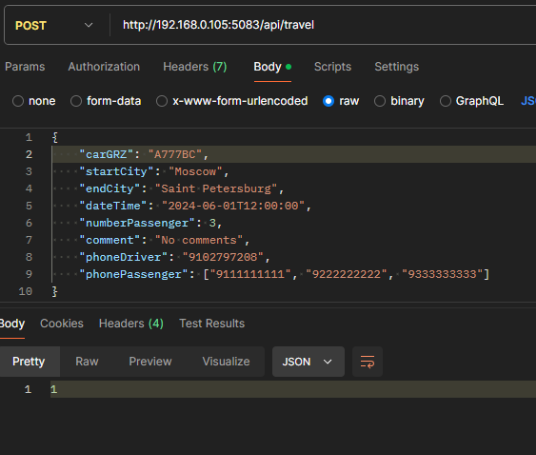
\includegraphics[width=0.7\linewidth]{images/test5}
	\caption{Тестирование запроса на создание поездки}
	\label{fig:test5}
\end{figure}

\begin{figure}[H]
	\centering
	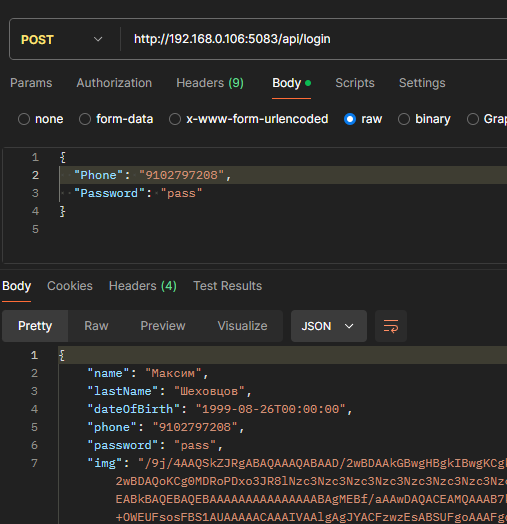
\includegraphics[width=0.6\linewidth]{images/test1}
	\caption{Тестирование запроса на вход в систему}
	\label{fig:test1}
\end{figure}

\begin{figure}[H]
	\centering
	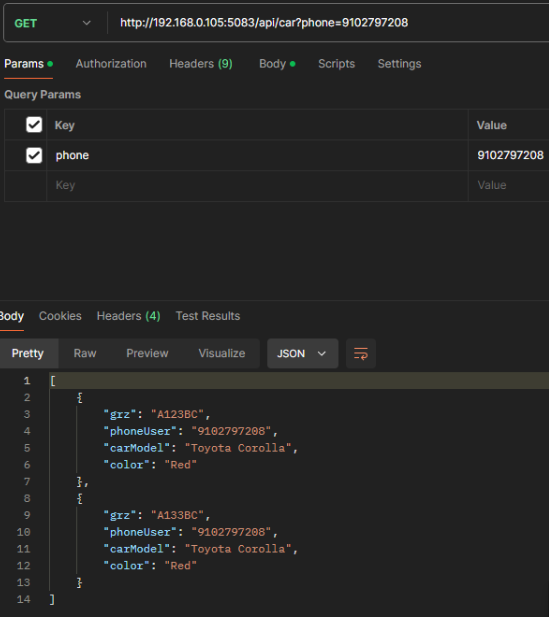
\includegraphics[width=0.6\linewidth]{images/test2}
	\caption{Тестирование запроса на получение автомобилей}
	\label{fig:test2}
\end{figure}

\begin{figure}[H]
	\centering
	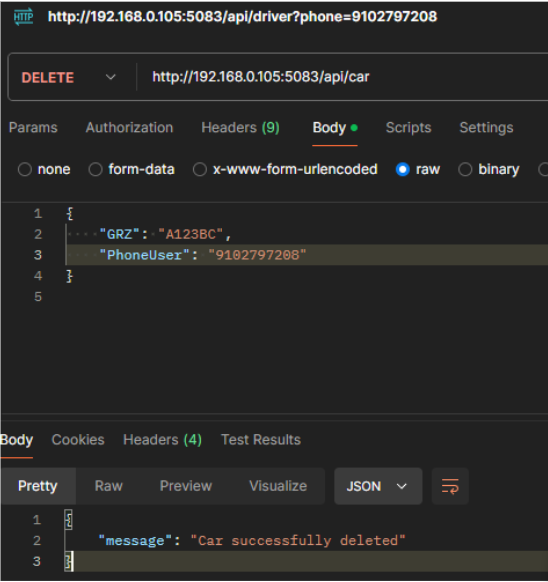
\includegraphics[width=0.7\linewidth]{images/test3}
	\caption{Тестирование запроса на удаление автомобиля}
	\label{fig:test3}
\end{figure}

\begin{figure}[H]
	\centering
	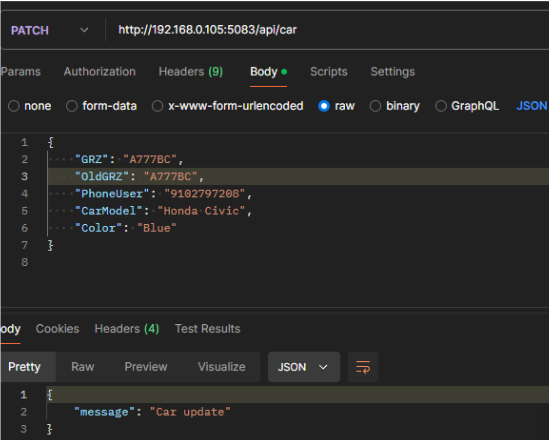
\includegraphics[width=0.7\linewidth]{images/test4}
	\caption{Тестирование запроса на изменение автомобиля}
	\label{fig:test4}
\end{figure}

\begin{figure}[H]
	\centering
	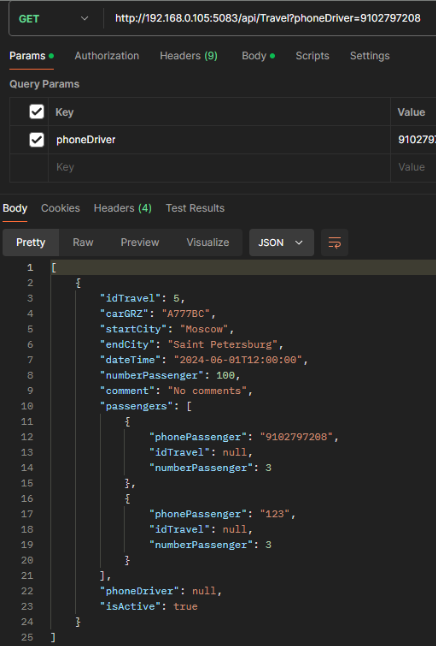
\includegraphics[width=0.8\linewidth]{images/test6}
	\caption{Тестирование запроса на получение водительских поездок}
	\label{fig:test6}
\end{figure}

\begin{figure}
	\centering
	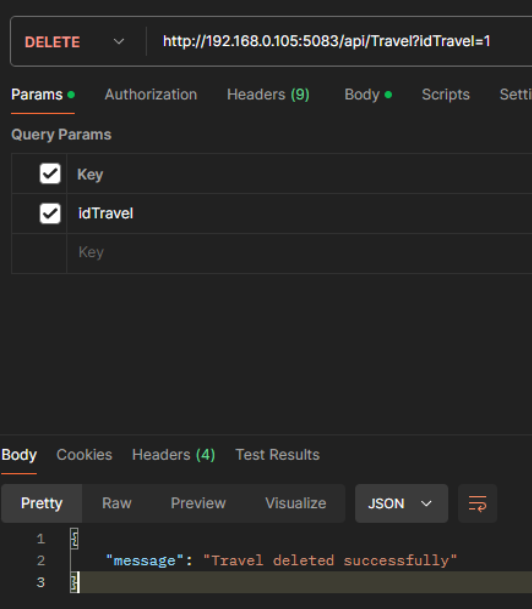
\includegraphics[width=0.9\linewidth]{images/test7}
	\caption{Тестирование запроса на удаление поездки}
	\label{fig:test7}
\end{figure}

\begin{figure}[H]
	\centering
	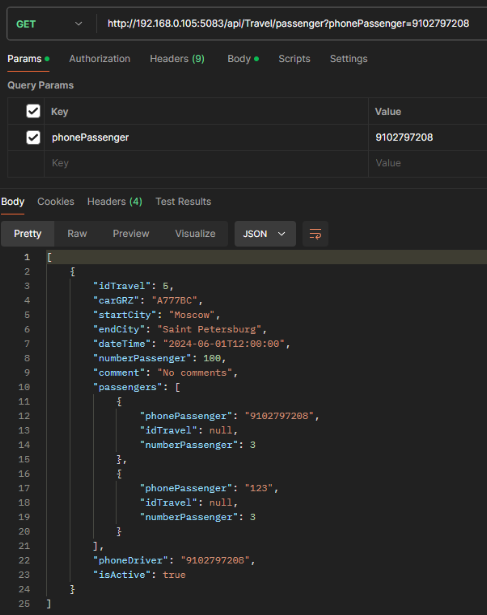
\includegraphics[width=0.9\linewidth]{images/test8}
	\caption{Тестирование запроса получение пассажирских поездок}
	\label{fig:test8}
\end{figure}

\begin{figure}[H]
	\centering
	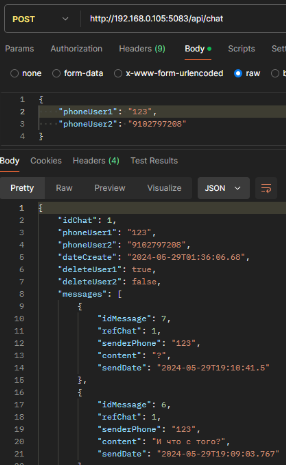
\includegraphics[width=0.8\linewidth]{images/test9}
	\caption{Тестирование запроса на получение пользовательских чатов}
	\label{fig:test9}
\end{figure}

\begin{figure}[H]
	\centering
	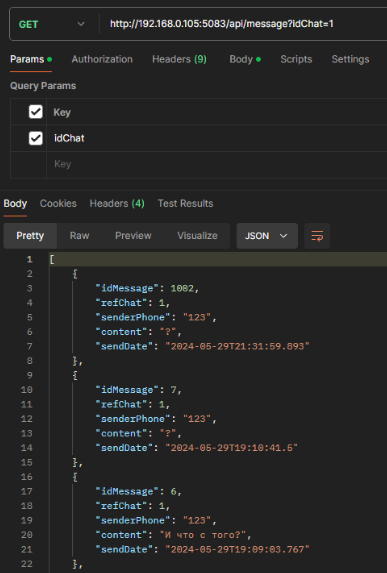
\includegraphics[width=0.8\linewidth]{images/test10}
	\caption{Тестирование запроса на получение сообщений по чату}
	\label{fig:test10}
\end{figure}

\begin{figure}[H]
	\centering
	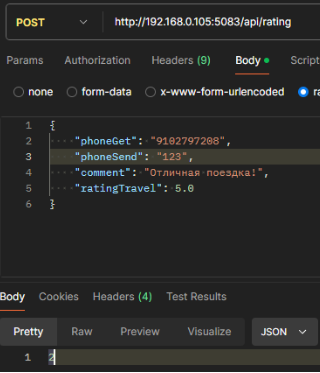
\includegraphics[width=0.7\linewidth]{images/test11}
	\caption{Тестирование запроса на создание комментария}
	\label{fig:test11}
\end{figure}
